\section{Related work}

\label{sec:related_work}

\begin{frame}{Building a deep image descriptor}

	Fully connected part of a the network is dropped and pooling is done on the last convolutional response:
	\vfill
	\begin{figure}
		\centering
		
\includegraphics[width=0.8\linewidth, trim = 2cm 0 0 0]{vect/MAC.pdf}			
	\end{figure}
	\vfill
	More complex aggregation methods exist: NetVLAD~\cite{Arandjelovic2017}, RMAC...
\end{frame}

\begin{frame}{Learning a deep image descriptor}

	\begin{minipage}{0.49\linewidth}
		\begin{minipage}[c]{0.26\linewidth}
			\uncover<1->{\includegraphics[width=\linewidth]{images/ex_query/anchor.png}}
			\vspace{0.1cm}
			\uncover<2->{\includegraphics[width=\linewidth]{images/ex_query/positive.png}}
			\vspace{0.1cm}
			\uncover<3>{\includegraphics[width=\linewidth]{images/ex_query/negative.png}}
		\end{minipage}
		\begin{minipage}{0.7\linewidth}
			\vfill
			\begin{figure}
				\centering
				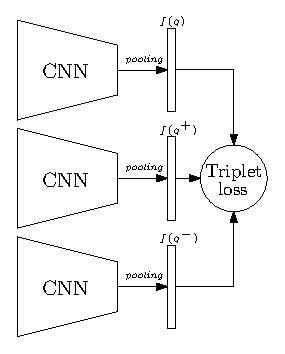
\includegraphics[width=\linewidth]{vect/triplet_loss.eps}			
			\end{figure}
			\vfill
		\end{minipage}
	\end{minipage}
	\begin{minipage}{0.48\linewidth}
		\begin{multline}
			\label{eq:triplet_loss}
			Loss_{triplet} = max\left( \norm{f(q) - f(q^+)}^2 - \right. \\
			\left. \norm{f(q) - f(q^-)}^2 + \lambda, 0\right),
		\end{multline}
		\vfill
		\begin{align*}
		with 
		\begin{cases}
				f(x) = \textnormal{descriptor of image $x$ } \\
				\lambda = \textnormal{triplet loss margin} \\
				q = \textnormal{query image} \\
				q^+ = \textnormal{positif example} \\
				q^- = \textnormal{negatif example} \\
		\end{cases}
		\end{align*}
	\end{minipage}
	
\end{frame}


\begin{frame}{Learning with side modality}
	\vfill
	Hallucination architecture from~\cite{Hoffman2016}, \textbf{never been applied to image description and VBL}.
	\vfill
	\begin{figure}
		\centering
		\only<1>{
			\includegraphics[width=0.70\linewidth, clip=true, trim = 0 0.5cm 8cm 0]{vect/training.pdf}			
		}
		\uncover<2>{
			\includegraphics[width=0.48\linewidth, clip=true, trim = 0 0.5cm 8cm 0]{vect/training.pdf}			
			\includegraphics[width=0.48\linewidth, clip=true, trim = 0 0.5cm 7.2cm 0]{vect/testing.pdf}
		}
	\end{figure}
	\only<1>{
		\centering
		Training
	}
	\only<2>{
		\centering
		\hspace{3.5cm} Deployment
	}	
	\vfill
\end{frame}
